\documentclass[10pt]{NSP1}

\usepackage{url,floatflt}
\usepackage{helvet,times}
\usepackage{psfig,graphics}
\usepackage{mathptmx,amsmath,amssymb,bm}
\usepackage{float}
\usepackage[bf,hypcap]{caption}
\usepackage[dvipsnames,table,xcdraw]{xcolor}
\usepackage{amsfonts}
\usepackage{graphicx}
\usepackage{subcaption}
\usepackage{upgreek}
\usepackage{placeins}
\usepackage{booktabs}
\usepackage{enumitem}

\usepackage{hyperref}





\topmargin=0.00cm

\def\sm{\smallskip}
\def\no{\noindent}

\usepackage{nccmath}
\ceqn                         % centred display equations, as in the original manuscript
\numberwithin{equation}{section}
\makeatletter
\let\oldtheequation\theequation
\renewcommand\tagform@[1]{\maketag@@@{\ignorespaces#1\unskip\@@italiccorr}}
\renewcommand\theequation{(\oldtheequation)}
\makeatother


% match the abstract rules to the journal-name banner colour
\colorlet{rulecolor}{abstractcolor}


\DeclareMathOperator{\sech}{sech}
\DeclareMathOperator{\csch}{csch}

\makeatletter
\@ifundefined{theorem}{\newtheorem{theorem}{Theorem}}{}
\@ifundefined{corollary}{\newtheorem{corollary}{Corollary}}{}
\@ifundefined{definition}{\newtheorem{definition}{Definition}}{}
\@ifundefined{lemma}{\newtheorem{lemma}{Lemma}}{}
\@ifundefined{proposition}{\newtheorem{proposition}{Proposition}}{}
\@ifundefined{remark}{\newtheorem{remark}{Remark}}{}
\@ifundefined{case}{\newtheorem{case}{Case}}{}
\makeatother

\def\firstpage{1}
\setcounter{page}{\firstpage}
\def\thevol{1}
\def\thenumber{1}
\def\theyear{2025}

\raggedbottom
\begin{document}

\titlefigurecaption{{\large \bf \rm Progress in Fractional Differentiation
and Applications}\\ {\it\small An International Journal}}

\title{Analytical soliton  of the ill-posed Boussinesq equation via a unified approach}

\author{Ali Akg\"ul$^{1,2,*}$, Farrah Ashraf$^{3}$, Rehan Khursheed$^{4}$, Romana Ashraf$^{3}$, M. Abdel-Aty$^{5,6,7}$ and M. Hafez$^{8,9}$}

\institute{Department of Electronics and Communication Engineering, Saveetha School of Engineering, SIMATS, Chennai, Tamilnadu, India\and
Siirt University, Art and Science Faculty, Department of Mathematics, 56100 Siirt, T\"urkiye\and
Department of Computer Science \& IT, The University of Lahore, Lahore, Pakistan\and
Department of Mathematics and Statistics, The University of Lahore, Lahore, Pakistan\and
College of Engineering and Computing, Liwa University, Abu Dhabi, United Arab Emirates\and
Deanship of Graduate Studies and Research, Ahlia University, P.O. Box 10878, Manama, Bahrain\and
Mathematics Department, Faculty of Science, Sohag University, P.O. Box 82524, Sohag, Egypt\and
Faculty of Engineering and Quantity Surveying, INTI International University Colleges, Nilai, Malaysia\and
Faculty of Management, Shinawatra University, Pathum Thani, Thailand}

\titlerunning{Analytical soliton  of the ill-posed Boussinesq equation}
\authorrunning{A. Akg\"ul et al.}

\mail{\parbox[t]{0.80\textwidth}{\raggedright f.as70000@gmail.com, rehankhursheed468@gmail.com, dr.romanauetian@gmail.com, amisaty@gmail.com, mohdahmed.hafez@newinti.edu.my}}

\received{}
\revised{}
\accepted{}
\published{}


\paperdoi{http://dx.doi.org/10.18576/pfda/120309}
\doi{http://dx.doi.org/10.18576/pfda/120309}
\abstracttext{In this paper, Unified approach method is proposed to construct more general precise (exact)  of ill-possed Boussinesq equation. This technique can be used to obtain the soliton  for the non-linear partial differential equation. This method can facilitate a deeper understanding of the wave phenomenon and also demonstrate the significance of researching different non-linear waves that occur in ocean engineering and physics. This technique has successfully provided several new solitons for ill-possed Boussinesq equation like Dark soliton, Kink shaped soliton, Periodic soliton and Dispersion-less soliton. Appropriate values are given to the parameters involved in the  of the equation for graphical view of our results. Our results show the efficiency and favor-ability of unified approach method for solving other non-linear partial differential equations.}

\keywords{Unified approach method, Analytical soliton , ill-posed Boussinesq equation, Kink shaped soliton, Singular soliton and Periodic soliton .}

\maketitle

\section{Introduction}
\noindent One of the most helpful subject in the literature is the study of accurate  to equations (differential). It is also crucial for explanation of many ambiguous subjects in applied science and engineering. The Boussinesq approximation is applied to water waves in fluid dynamics. It is an approximation that works for waves that are long and weakly non-linear. The approximation bears Joseph Boussinesq's name who derived it initially in response to the observation of the translational wave by  John Scott Russell. The Boussinesq equations were first presented in a publication by Boussinesq in 1872. In contrast to the equations for shallow water, the Boussinesq equations account for frequency dispersion. These equations take into account how wave frequency affects wave behavior that the shallow water equations do not account for. The solitons obtained from Boussinesq equations can either create a singularity in a finite amount of time or decay when perturbed which means that they gradually diminishes in stability when disrupted. It is likely that one would consider the Boussinesq equation to be very unique in and of itself. But in-fact, it is a physiologically meaningful equation that represents a non-linear integrable generalization of the wave equation. With the KdV equation being the most basic it is also a typical illustration of dimensional reduction within the context of the KP hierarchy. Many characteristics in fluid systems, signal processing, non-linear systems, plasma physics, fluid dynamics, electricity, science and engineering are modeled by non -linear partial equations.\\
The Boussinesq equation is a fundamental generalized wave equation that arises in fluid mechanics and plasma physics and describes the propagation of small amplitude long waves in shallow water is viewed as
\begin{eqnarray}
u_{tt}-u_{xx}-\beta(u^2)_{xx}-\gamma u_{xxxx}=0,
\end{eqnarray}
where $\beta$ is the non-linear parameter representing the depth of the fluid, $\gamma$ is the characteristic speed of the long wave and \emph{u (x, t)} is the elevation of the free surface of the fluid. \emph{x} and \emph{t} are the scaled spatial and temporal variables respectively.\\
Finding accurate  to partialequations (differential) is a significant research in the context of science and engineering. Different methods can be adopted to find the accurate solution to the non-linear partial differential equations. Well-known techniques for employing computational models and programs like Maple to find optimal  to non-physical problems have been applied to recent work in the past several years. These techniques or methods are as follows: Method of Homotopy perturbation \cite{A1}, Method of variational iteration \cite{A2}, Method of The $G/G^{'}$ - Expansion \cite{A3,a4,a5}, The method of Exp-Function \cite{a6,a7,a8,a9}, Method of Modified simple equation \cite{a10,a11}, Method of tanh function \cite{a12,a13,a14}, Method of Kudryashov \cite{a15,a16}, Method of The Trial equation \cite{a17}, Method of the Backscatter \cite{a18}, Backlund transform\cite{a19}, Method of Hirota bilinear \cite{a20}, Homogeneous balance method\cite{a21} and Method of Jacobi and Weierstrass elliptic function \cite{a22} etc. One of the finest ways to get the precise answers to the (NLPDE's) non-linear partial differential equations is to use the Unified Approach Technique. This approach will be used in this study to show how the ill-posed Boussinesq problem behaves and to determine its precise solution. Numerous precise  to the ill-posed Boussinesq problem can be found using this method with different shapes of solitons like Periodic, Kink, Singular, Dispersion-less and Dark solitons.
\section{Unified Approach Method }
The methodology of unified approach method has the following steps:
\subsection{Different Steps of the Unified Approach method}
\textbf{Step 1:}
We use the traveling wave transformation equation to convert
\begin{eqnarray}\label{PDE}
\Omega(u_x,u_t,u_{xt},u_{xx},u_{xxx}........)=0,
\end{eqnarray}
into ODE form (By combining the variables we get)
\begin{eqnarray}\label{ODE}
\Pi(U',U'',U''',.............)=0.
\end{eqnarray}\\
\textbf{Step 2:}
 We now examine the solution of Eq. \ref{ODE} which takes the following form
\begin{eqnarray}\label{TF}
\frac{d}{d \zeta}\eta \! \left(\zeta \right) =H_{0}+ \sum_{j=1}^M H_{j}\eta \left(\zeta \right)^{j}+\sum_{j=1}^M \frac{F_{j}}{\eta \left(\zeta \right)^{j}}.
\end{eqnarray}
\textbf{Step 3:}
We may now calculate the value of M by balancing the highest order derivative term in Eq. \ref{ODE} with the highest order non-linear term.\\
Reccati Equation of the form:
\begin{eqnarray}\label{RE}
\frac{d}{d \zeta}\eta \! \left(\zeta \right) =\eta \! \left(\zeta \right)^{2}+N.
\end{eqnarray}
Here we have different families ${\eta(\zeta)}$ of Eq. \ref{RE} depending upon the value of \emph{N} (The value of \emph{N} can be Zero, negative and positive). \\
\textbf{when $\textbf{ N $<$ 0} $ }
\begin{align}\label{FAM1}
\begin{cases}\\\
\textbf{(i)}\quad \eta \! \left(\zeta \right) =\frac{-\sqrt{-\left(P^{2}+Q^{2}\right) N}-P \sqrt{-N}\, \cosh \, \left(2 \sqrt{-N}\, \left(\zeta +\psi \right)\right)}{P \sinh \, \left(2 \sqrt{-N}\, \left(\zeta +\psi \right)\right)+Q},\\\
\textbf{(ii)}\quad \eta \! \left(\zeta \right) =\frac{\sqrt{-\left(P^{2}+Q^{2}\right) N}-P \sqrt{-N}\, \cosh \, \left(2 \sqrt{-N}\, \left(\zeta +\psi \right)\right)}{P \sinh \, \left(2 \sqrt{-N}\, \left(\zeta +\psi \right)\right)+Q},\\\
\textbf{(iii)}\quad \eta \! \left(\zeta \right) =-\sqrt{-N}+\frac{2 P \sqrt{-N}}{P +\cosh \, \left(2 \sqrt{-N}\, \left(\zeta +\psi \right)\right)-\sinh \, \left(2 \sqrt{-N}\, \left(X +\psi \right)\right)},\\\
\textbf{(iv)}\quad \eta \! \left(\zeta \right) =\sqrt{-N}+\frac{2 P \sqrt{-N}}{P +\cosh \, \left(2 \sqrt{-N}\, \left(\zeta +\psi \right)\right)-\sinh \, \left(2 \sqrt{-N}\, \left(X +\psi \right)\right)}.\\
\end{cases}
\end{align}
\textbf{when $\textbf{ N $>$ 0} $ }
\begin{align}\label{FAM2}
\begin{cases}\\\
\textbf{(i)}\quad \eta \! \left(\zeta \right) =\frac{-\sqrt{\left(P^{2}+Q^{2}\right) N}-P \sqrt{N}\, \cos \, \left(2 \sqrt{N}\, \left(\zeta +\psi \right)\right)}{P \sin \, \left(2 \sqrt{N}\, \left(\zeta +\psi \right)\right)+Q},\\\
\textbf{(ii)}\quad \eta \! \left(\zeta \right) =\frac{\sqrt{\left(P^{2}+Q^{2}\right) N}-P \sqrt{N}\, \cos \, \left(2 \sqrt{N}\, \left(\zeta +\psi \right)\right)}{P \sin \, \left(2 \sqrt{N}\, \left(\zeta +\psi \right)\right)+Q},\\\
\textbf{(iii)}\quad \eta \! \left(\zeta \right) =-i \sqrt{N}+\frac{2 i P \sqrt{N}}{P +\cos \, \left(2 \sqrt{N}\, \left(\zeta +\psi \right)\right)-i \sin \, \left(2 \sqrt{N}\, \left(\zeta +\psi \right)\right)},\\\
\textbf{(iv)}\quad \eta \! \left(\zeta \right) =i \sqrt{-N}+\frac{2 i P \sqrt{N}}{P +\cos \, \left(2 \sqrt{N}\, \left(\zeta +\psi \right)\right)-i \sin \, \left(2 \sqrt{N}\, \left(X +\psi \right)\right)}.\\
\end{cases}
\end{align}
\textbf{when $\textbf{ N $=$ 0}$ }
\begin{eqnarray}\label{FAM3}
\quad \eta \! \left(\zeta \right) = -\frac{1}{\zeta +\psi}.
\end{eqnarray}
\section{Solving the ill-posed Boussinesq Equation}

Non-linear ill-posed Boussinesq equation of the form
\begin{eqnarray}\label{PDE1}
u_{\mathit{tt}} =u_{\mathit{xx}}+\left(u^{2}\right)_{\mathit{xx}}+u_{\mathit{xxxx}},
\end{eqnarray}
Using the transformation
\begin{eqnarray}\label{TF1}
u(x,t)=U(\zeta), \qquad \zeta=x - v t.
\end{eqnarray}
in Eq. \ref{PDE1} and integrating the result twice we get our required ODE form of ill-posed Boussinesq equation
\begin{eqnarray}\label{ODE1}
\left(v^{2}-1\right) U -U^{2}-U'' = 0.
\end{eqnarray}
We now obtain \emph{M = 2} by applying the Homogeneous Balancing Principle, which involves balancing the maximum degree non-linear term $U^{2}$ with the maximum order derivative term $U_{\zeta \zeta}$.\\\\
Now by replacing $M=2$ in equation in Eq. \ref{TF} we get
\begin{eqnarray}\label{S}
U  \left(\zeta \right) =H_{0}+H_{1} \eta  \left(\zeta \right)+H_{2} \eta  \left(\zeta \right)^{2}+\frac{F_{1}}{\eta \! \left(\zeta \right)}+\frac{F_{2}}{\eta  \left(\zeta \right)^{2}}.
\end{eqnarray}
here we need to find the constants involved in $U{(\zeta)}$ which are $H_{0}$, $H_{1}$, $H_{2}$, $F_{1}$ and $F_{2}$,
The $\eta{(\zeta)}$ represents (the families given) the  of Eq. \ref{RE}.\\
Now substitute Eq. \ref{RE} and Eq. \ref{S} in Eq. \ref{ODE1} then simplify resulting equation to get the coefficients of all powers of ${\eta(\zeta)}$ and set all the coefficients of the various powers of $\eta{(\zeta)}$ to zero to produce a set of simultaneous solvable algebraic equations.
The coefficients of different powers of $\eta{(\zeta)}$ are as follows\\
\begin{align}
\begin{cases}
\eta{(\zeta)}^{-4} :\;\;\;\quad -2 F_{1} N^{2}-2 F_{1} F_{2}=0, \\\
\eta{(\zeta)}^{-3} :\;\,\quad -2 F_{1} N^{2}-2 F_{1} F_{2}=0, \\\
\eta{(\zeta)}^{-2} :\;\,\quad F_{2} v^{2}-8 F_{2} N -F_{1}^{2}-2 H_{0} F_{2}-F_{2}=0,\\\
\eta{(\zeta)}^{-1} :\,\;\quad v^{2} F_{1}-2 N F_{1}-2 F_{1} H_{0}-2 F_{2} H_{1}-F_{1}=0, \\\
\eta{(\zeta)}^{0}  :\qquad -2 H_{2} N^{2}+H_{0} v^{2}-2 H_{1} F_{1}-2 H_{2} F_{2}-H_{0}^{2}-2 F_{2}-H_{0}=0,\\\
\eta{(\zeta)}^{1}  :\qquad H_{1} v^{2}-2 H_{1} N -2 H_{2} F_{1}-2 H_{0} H_{1}-H_{1}=0, \\\
\eta{(\zeta)}^{2}  :\qquad v^{2} H_{2}-8 N H_{2}-2 H_{0} H_{2}-H_{1}^{2}-H_{2}=0, \\\
\eta{(\zeta)}^{3}  :\qquad-2 H_{1} H_{2}-2 H_{1}=0, \\\
\eta{(\zeta)}^{4}  :\qquad-H_{2}^{2}-6 H_{2}=0.\\
\end{cases}
\end{align}
Now by using Maple software we find the simultaneous solution of these equations.\\
\textbf{Set I:}
\begin{eqnarray}\label{set1}
v = \sqrt{16 N -1},\,F_{1} = 0,\,F_{2} = -6 N^{2},\, H_{0} = -12 N,\, H_{1} = 0\,{\&}\,H_{2} = -6.
\end{eqnarray}
\textbf{Solution of Set I:}\\
By substituting Eq. \ref{TF1}, Eq. \ref{set1} and using \textbf{(iv)} from Eq. \ref{FAM1}, \textbf{(v,vii)} from Eq. \ref{FAM2} and Eq. \ref{FAM3} in Eq. \ref{S} we will get the following .
\begin{eqnarray}\label{U1}
U_{1} \left(\zeta \right) =H_{0}+\frac{H_{2} \left[\sqrt{\left(P^{2}+Q^{2}\right) N}-P \sqrt{N}\, \cos \! \left(2 \sqrt{N}\, \left(-v t +\psi +x \right)\right)\right]}{P \sin \! \left(2 \sqrt{N}\, \left(-v t +\psi +x \right)\right)+Q}+\nonumber
\end{eqnarray}
\begin{eqnarray}
\frac{F_{2} \left[P \sin \! \left(2 \sqrt{N}\, \left(-v t +\psi +x \right)\right)+Q \right]^{2}}{{\left[\sqrt{\left(P^{2}+Q^{2}\right) N}-P \sqrt{N}\, \cos \! \left(2 \sqrt{N}\, \left(-v t +\psi +x \right)\right)\right]}^{2}}.
\end{eqnarray}
\begin{eqnarray}\label{U2}
U_{2} \left(\zeta \right) =
H_{0}+\frac{H_{2} \left[-\sqrt{\left(P^{2}+Q^{2}\right) N}-P \sqrt{N}\, \cos \! \left(2 \sqrt{N}\, \left(-v t +\psi +x \right)\right)\right]}{P \sin \! \left(2 \sqrt{N}\, \left(-v t +\psi +x \right)\right)+Q}+\nonumber
\end{eqnarray}
\begin{eqnarray}
\frac{F_{2} \left[P \sin \! \left(2 \sqrt{N}\, \left(-v t +\psi +x \right)\right)+Q \right]^{2}}{{\left[-\sqrt{\left(P^{2}+Q^{2}\right) N}-P \sqrt{N}\, \cos \! \left(2 \sqrt{N}\, \left(-v t +\psi +x \right)\right)\right]}^{2}}.
\end{eqnarray}
\begin{eqnarray}\label{U3}
U_{3} \left(\zeta \right) =
H_{0}+H_{2} \left[\sqrt{-N}+\frac{2 P \sqrt{-N}}{P +\cosh \! \left(2 \sqrt{-N}\, \left(-v t +\psi +x \right)\right)-\sinh \! \left(2 \sqrt{-N}\, \left(-v t +\psi +x \right)\right)}\right]+\nonumber
\end{eqnarray}
\begin{eqnarray}
\frac{F_{2}}{\left[\sqrt{-N}+\frac{2 P \sqrt{-N}}{P +\cosh \left(2 \sqrt{-N}\, \left(-v t +\psi +x \right)\right)-\sinh \left(2 \sqrt{-N}\, \left(-v t +\psi +x \right)\right)}\right]^{2}}.
\end{eqnarray}
\begin{eqnarray}\label{U4}
U_{4}\left(\zeta \right) =H_{0}-\frac{H_{2}}{-v t +\psi +x}+F_{2} \left(-v t +\psi +x \right)^{2}.
\end{eqnarray}
\textbf{Set II:}
\begin{eqnarray}\label{set2}
v = \sqrt{-4 N -1},\,F_{1} = 0,\,F_{2} = -6 N^{2},\, H_{0} = -2 N,\, H_{1} = 0\,{\&}\, H_{2} = 0.
\end{eqnarray}
By substituting Eq. \ref{TF1}, Eq. \ref{set2} and using Eq. \ref{FAM1}, \ref{FAM3} in Eq. \ref{S} we will get the following .\\
\textbf{Solution of Set II:}\\\
\begin{eqnarray}\label{U11}
U_{1}\! \left(\zeta \right) =H_{0}+\frac{F_{2} \left[P \sinh \! \left(2 \sqrt{-N}\, \left(-v t +\psi +x \right)\right)+Q \right]}{\sqrt{-\left(P^{2}+Q^{2}\right) N}-P \sqrt{-N}\, \cosh \! \left(2 \sqrt{-N}\, \left(-v t +\psi +x \right)\right)}.
\end{eqnarray}
\begin{eqnarray}\label{U22}
U_{2}\! \left(\zeta \right) =H_{0}+\frac{F_{2} \left[P \sinh \! \left(2 \sqrt{-N}\, \left(-v t +\psi +x \right)\right)+Q \right]}{-\sqrt{-\left(P^{2}+Q^{2}\right) N}-P \sqrt{-N}\, \cosh \! \left(2 \sqrt{-N}\, \left(-v t +\psi +x \right)\right)}.
\end{eqnarray}
\begin{eqnarray}\label{U33}
U_{3}\! \left(\zeta \right) =H_{0}+\frac{F_{2}}{\sqrt{-N}+\frac{2 P \sqrt{-N}}{P +\cosh \left(2 \sqrt{-N}\, \left(-v t +\psi +x \right)\right)-\sinh \left(2 \sqrt{-N}\, \left(-v t +\psi +x \right)\right)}}.
\end{eqnarray}
\begin{eqnarray}\label{U44}
U_{4}\! \left(\zeta \right) =H_{0}+\frac{F_{2}}{-\sqrt{-N}+\frac{2 P \sqrt{-N}}{P +\cosh \left(2 \sqrt{-N}\, \left(-v t +\psi +x \right)\right)-\sinh \left(2 \sqrt{-N}\, \left(-v t +\psi +x \right)\right)}}.
\end{eqnarray}
\begin{eqnarray}\label{U55}
U_{5}\! \left(\zeta \right) = H_{0}+F_{2} \left(v t -\psi -x \right).
\end{eqnarray}
\textbf{Set III:}
\begin{eqnarray}\label{set3}
v = \sqrt{-16 N -1},\,F_{1} = 0,\,F_{2} = -6 N^{2},\, H_{0} = 4 N,\, H_{1} = 0,\,{\&}\, H_{2} = -6.
\end{eqnarray}
\textbf{Solution of Set III:}\\
By substituting Eq. \ref{TF1}, Eq. \ref{set3} and using Eq. \ref{FAM1}, \ref{FAM3} in Eq. \ref{S} we will get the following .\\
\begin{eqnarray}\label{U111}
U_{1}\ \left(\zeta \right) = H_{0}+H_{2} \left[\sqrt{-N}+\frac{2 P \sqrt{-N}}{P +\cosh \! \left(2 \sqrt{-N}\,
\left(-t v +\psi +x \right)\right)-\sinh \! \left(2 \sqrt{-N}\, \left(-t v +\psi +x \right)\right)}\right]^{2}+\nonumber
\end{eqnarray}
\begin{eqnarray}
\frac{F_{2}}{\left[\sqrt{-N}+\frac{2 P \sqrt{-N}}{P +\cosh \left(2 \sqrt{-N}\, \left(-t v +\psi +x \right)\right)-\sinh \left(2 \sqrt{-N}\,
\left(-t v +\psi +x \right)\right)}\right]^{2}}.
\end{eqnarray}
\begin{eqnarray}\label{U222}
U_{2}\! \left(\zeta \right) =
H_{0}+H_{2} \left[-\sqrt{-N}+\frac{2 P \sqrt{-N}}{P +\cosh \! \left(2 \sqrt{-N}\, \left(-t v +\psi +x \right)\right)-\sinh \! \left(2 \sqrt{-N}\, \left(-t v +\psi +x \right)\right)}\right]^{2}+\nonumber
\end{eqnarray}
\begin{eqnarray}
\frac{F_{2}}{\left[-\sqrt{-N}+\frac{2 P \sqrt{-N}}{P +\cosh \left(2 \sqrt{-N}\, \left(-t v +\psi +x \right)\right)-\sinh \left(2 \sqrt{-N}\, \left(-t v +\psi +x \right)\right)}\right]^{2}}.
\end{eqnarray}
\begin{eqnarray}\label{U333}
U_{3}\! \left(\zeta \right) =
H_{0}+\frac{H_{2} {\left[\sqrt{-\left(P^{2}+Q^{2}\right) N}-P \sqrt{-N}\, \cosh \! \left(2 \sqrt{-N}\, \left(-t v +\psi +x \right)\right)\right]}^{2}}{\left[P \sinh \! \left(2 \sqrt{-N}\, \left(-t v +\psi +x \right)\right)+Q \right]^{2}}+\nonumber
\end{eqnarray}
\begin{eqnarray}
\frac{F_{2} \left[P \sinh \! \left(2 \sqrt{-N}\, \left(-t v +\psi +x \right)\right)+Q \right]^{2}}{{\left[\sqrt{-\left(P^{2}+Q^{2}\right) N}-P \sqrt{-N}\, \cosh \! \left(2 \sqrt{-N}\, \left(-t v +\psi +x \right)\right)\right]}^{2}}.
\end{eqnarray}
\begin{eqnarray}\label{U444}
U_{4}\! \left(\zeta \right) =
H_{0}+\frac{H_{2} {\left[-\sqrt{-\left(P^{2}+Q^{2}\right) N}-P \sqrt{-N}\, \cosh \! \left(2 \sqrt{-N}\, \left(-t v +\psi +x \right)\right)\right]}^{2}}{\left[P \sinh \! \left(2 \sqrt{-N}\, \left(-t v +\psi +x \right)\right)+Q \right]^{2}}+\nonumber
\end{eqnarray}
\begin{eqnarray}
\frac{F_{2} \left[P \sinh \! \left(2 \sqrt{-N}\, \left(-t v +\psi +x \right)\right)+Q \right]^{2}}{{\left[-\sqrt{-\left(P^{2}+Q^{2}\right) N}-P \sqrt{-N}\, \cosh \! \left(2 \sqrt{-N}\, \left(-t v +\psi +x \right)\right)\right]}^{2}}.
\end{eqnarray}
\begin{eqnarray}\label{U555}
U_{5}\! \left(\zeta \right) =
H_{0}+\frac{H_{2}}{\left(-t v +\psi +x \right)^{2}}+F_{2} \left(-t v +\psi +x \right)^{2}.
\end{eqnarray}
\newpage
\FloatBarrier
\section{The Graphical Representation of sets}
\textbf{Graphical Representation of the Set I:}\\\
By substituting ${N=0.2}$, \,${P=0.021}$, \,${Q=397}$ and \,${\psi=3}$ different forms of soliton waves are observed via 3D and wave propagates in an interval as shown in figure.\\
\begin{figure}[h!]\label{A1}
    \centering
    \begin{tabular}{ccc}
        \begin{minipage}{.30\textwidth} 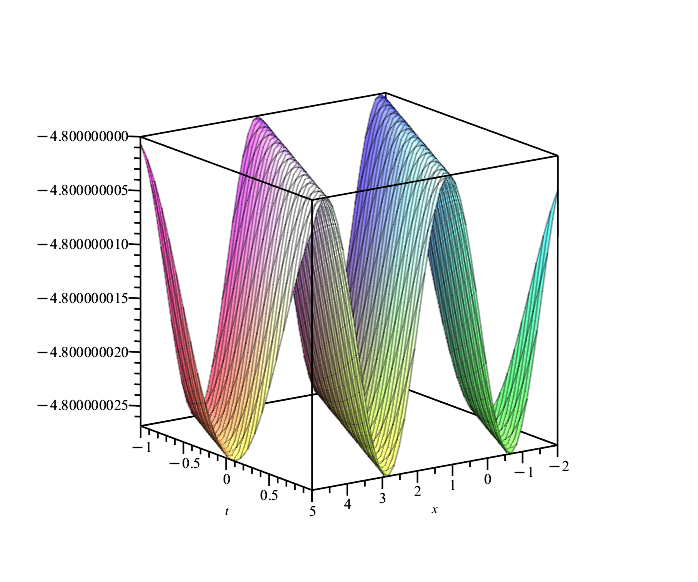
\includegraphics[width=\linewidth,
            height=35mm]{u1.png}\subcaption{} \end{minipage} & \begin{minipage}{.30\textwidth}
            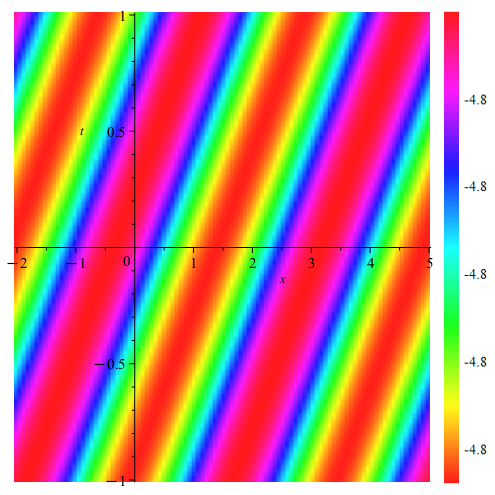
\includegraphics[width=\linewidth, height=35mm]{d1.png}\subcaption{} \end{minipage}
    \end{tabular}%
 \noindent\caption{\ref{U1} yields the 3D and density plot of $U_1(\xi)$ which are displayed here.}\label{F1}
\end{figure}\\
\begin{figure}[h!]
    \centering
    \begin{tabular}{ccc}
        \begin{minipage}{.30\textwidth} 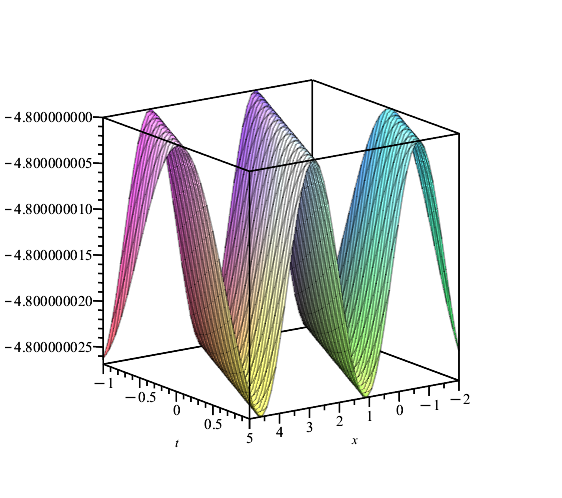
\includegraphics[width=\linewidth,
            height=35mm]{u2.png}\subcaption{} \end{minipage} & \begin{minipage}{.30\textwidth}
            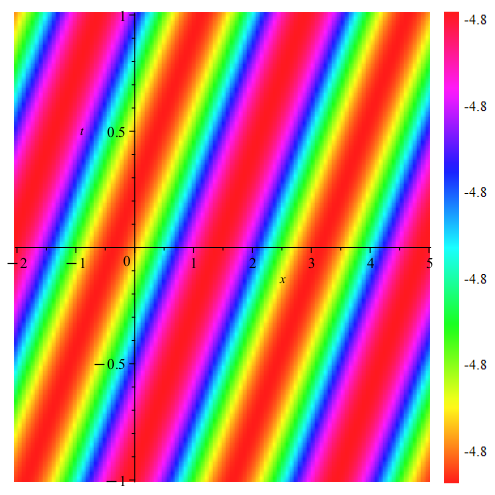
\includegraphics[width=\linewidth, height=35mm]{d2.png}\subcaption{} \end{minipage}
    \end{tabular}%
 \noindent\caption{\ref{U2} yields the 3D and density plot of $U_2(\xi)$ which are displayed here.}\label{F2}
\end{figure}\\
\begin{figure}[h!]
    \centering
    \begin{tabular}{ccc}
        \begin{minipage}{.30\textwidth} 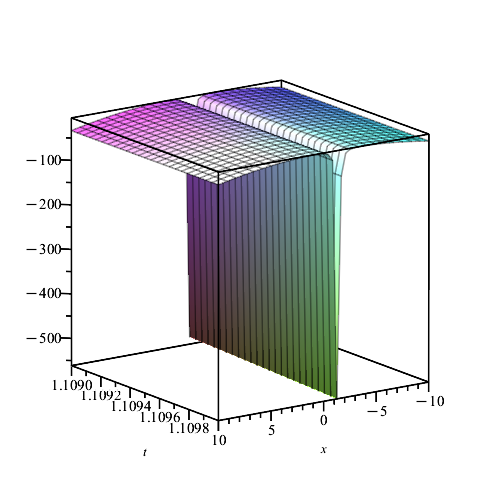
\includegraphics[width=\linewidth,
            height=35mm]{u3.png}\subcaption{} \end{minipage} & \begin{minipage}{.30\textwidth}
            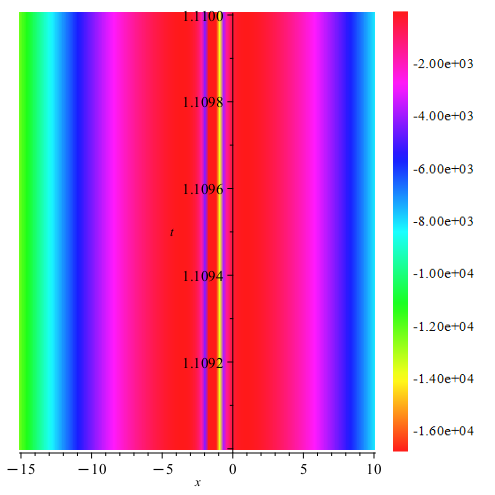
\includegraphics[width=\linewidth, height=35mm]{d3.png}\subcaption{} \end{minipage}
    \end{tabular}%
 \noindent\caption{\ref{U4} yields the 3D and density plot of $U_4(\xi)$ which are displayed here.}\label{F3}
\end{figure}
\FloatBarrier
\textbf{Graphical Representation of the Set II:}\\\
By substituting ${N=-0.3}$, \,${P=0.021}$, \,${Q=397}$ and \,${\psi=3}$ we get different soliton waves observed via 3D and wave propagates in an interval as shown in figure.\\
\begin{figure}[h!]
    \centering
    \begin{tabular}{ccc}
        \begin{minipage}{.30\textwidth} 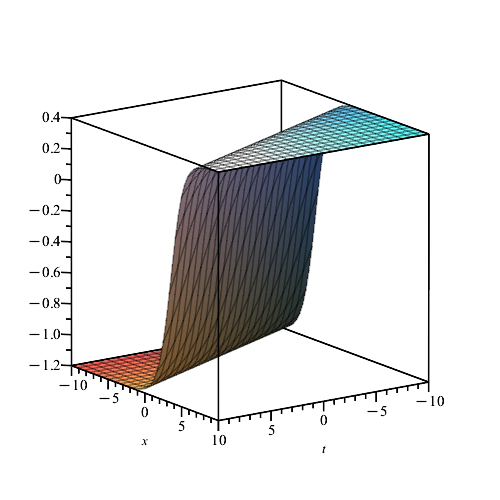
\includegraphics[width=\linewidth,
            height=35mm]{u4.png}\subcaption{} \end{minipage} & \begin{minipage}{.30\textwidth}
            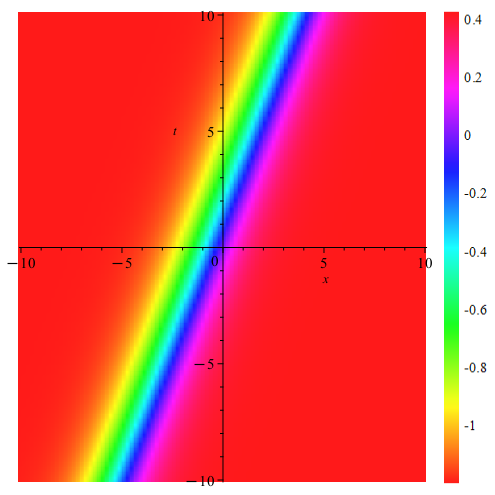
\includegraphics[width=\linewidth, height=35mm]{d4.png}\subcaption{} \end{minipage}
    \end{tabular}%
 \noindent\caption{\ref{U33} yields the 3D and density plot of $U_3(\xi)$ which are displayed here.}\label{F4}
\end{figure}\\
\begin{figure}[h!]\label{A1}
    \centering
    \begin{tabular}{ccc}
        \begin{minipage}{.30\textwidth} 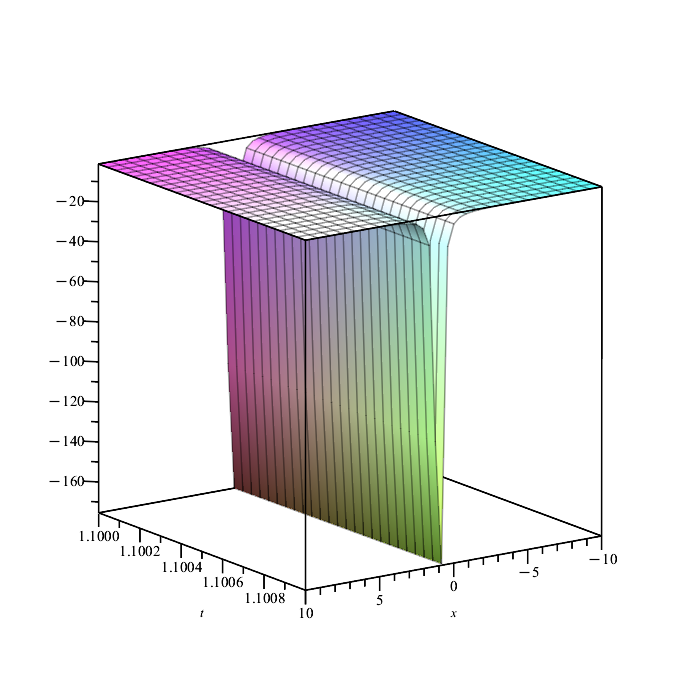
\includegraphics[width=\linewidth,
            height=35mm]{u5.png}\subcaption{} \end{minipage} & \begin{minipage}{.30\textwidth}
            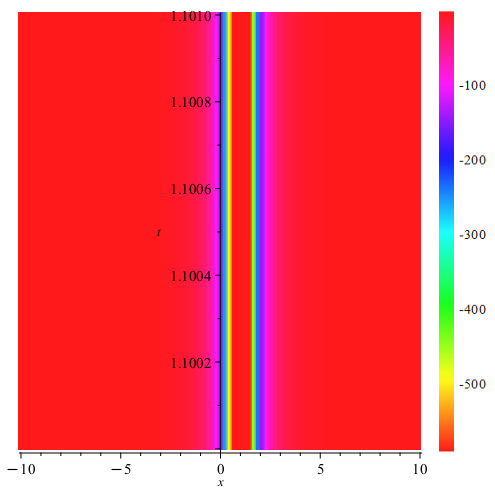
\includegraphics[width=\linewidth, height=35mm]{d5.png}\subcaption{} \end{minipage}
    \end{tabular}%
 \noindent\caption{\ref{U44} yields the 3D and density plot of $U_4(\xi)$ which are displayed here.}\label{F5}
\end{figure}\\
\begin{figure}[h!]
    \centering
    \begin{tabular}{ccc}
        \begin{minipage}{.30\textwidth} 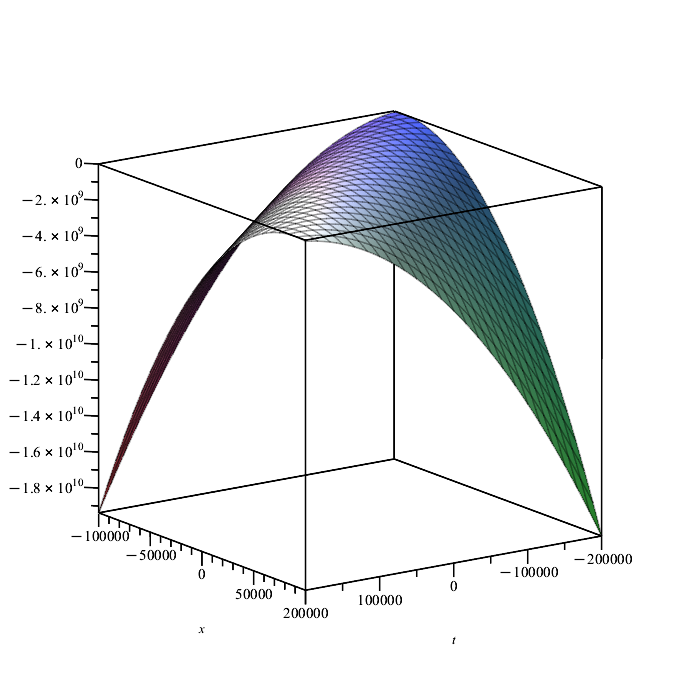
\includegraphics[width=\linewidth,
            height=40mm]{u6.png}\subcaption{} \end{minipage} & \begin{minipage}{.30\textwidth}
            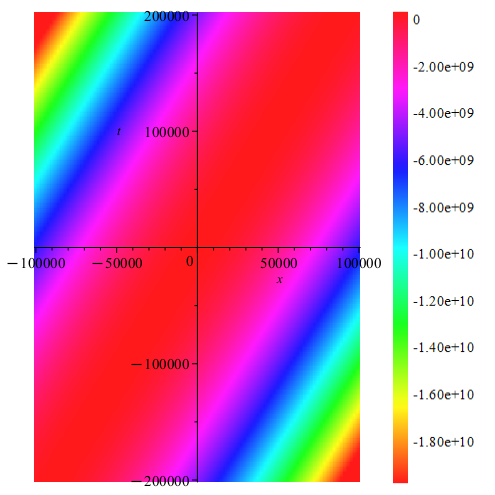
\includegraphics[width=\linewidth, height=40mm]{d6.png}\subcaption{} \end{minipage}
    \end{tabular}%
 \noindent\caption{\ref{U55} yields the 3D and density plot of $U_5(\xi)$ which are displayed here.}\label{F6}
\end{figure}
\FloatBarrier
\textbf{Graphical Representation of the Set III:}\\\
By substituting ${N=-0.2}$, \,${P=0.021}$, \,${Q=397}$ and \,${\psi=3}$ different forms of soliton waves are observed via 3D and wave propagates in an interval as shown in figure.\\
\begin{figure}[h!]\label{A1}
    \centering
    \begin{tabular}{ccc}
        \begin{minipage}{.30\textwidth} 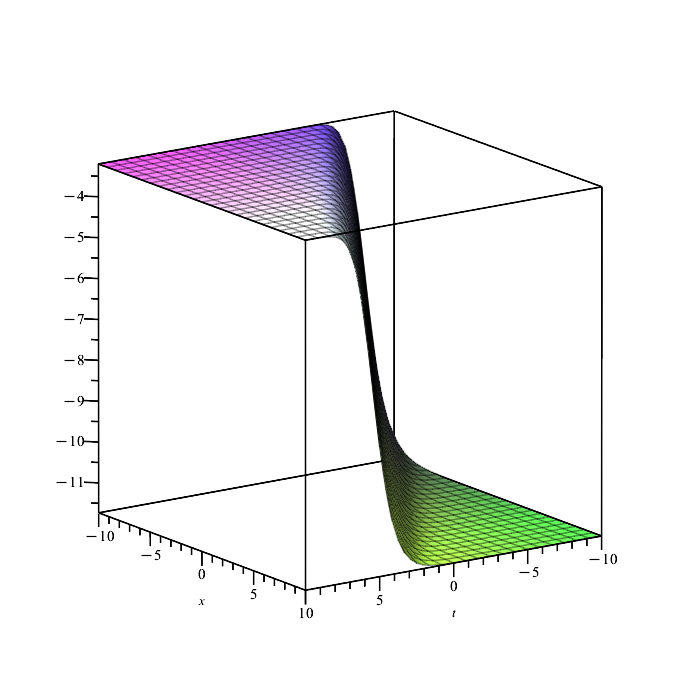
\includegraphics[width=\linewidth,
            height=35mm]{u7.png}\subcaption{} \end{minipage} & \begin{minipage}{.30\textwidth}
            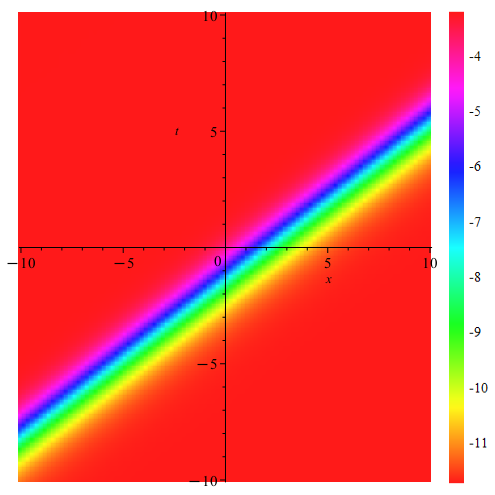
\includegraphics[width=\linewidth, height=35mm]{d7.png}\subcaption{} \end{minipage}
    \end{tabular}%
 \noindent\caption{\ref{U111} yields the 3D and density plot of $U_1(\xi)$ which are displayed here.}\label{F7}
\end{figure}
\begin{figure}[h!]
    \centering
    \begin{tabular}{ccc}
        \begin{minipage}{.30\textwidth} 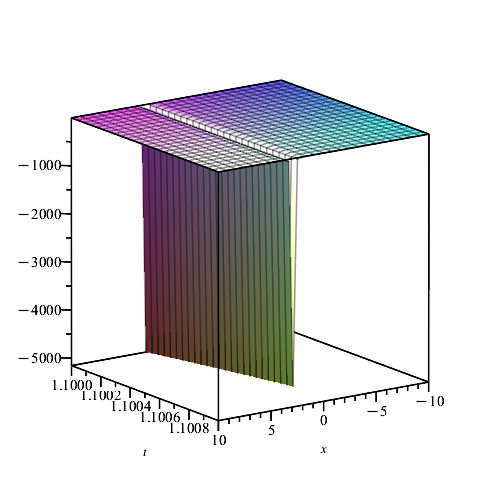
\includegraphics[width=\linewidth,
            height=35mm]{u8.png}\subcaption{} \end{minipage} & \begin{minipage}{.30\textwidth}
            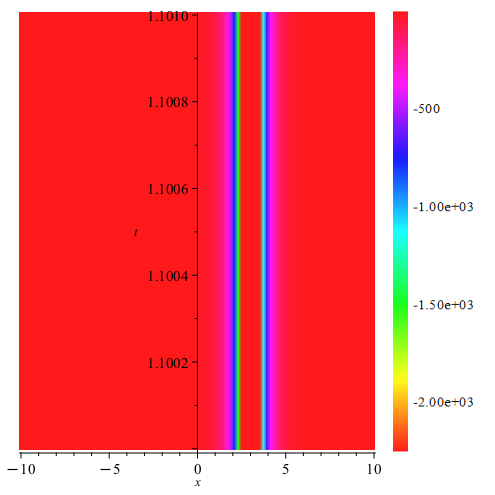
\includegraphics[width=\linewidth, height=35mm]{d8.png}\subcaption{} \end{minipage}
    \end{tabular}%
 \noindent\caption{\ref{U222} yields the 3D and density plot of $U_2(\xi)$ which are displayed here.}\label{F8}
\end{figure}
\begin{figure}[h!]
    \centering
    \begin{tabular}{ccc}
        \begin{minipage}{.30\textwidth} 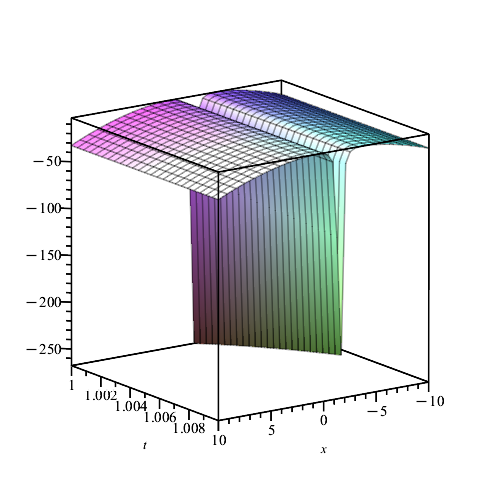
\includegraphics[width=\linewidth,
            height=35mm]{u9.png}\subcaption{} \end{minipage} & \begin{minipage}{.30\textwidth}
            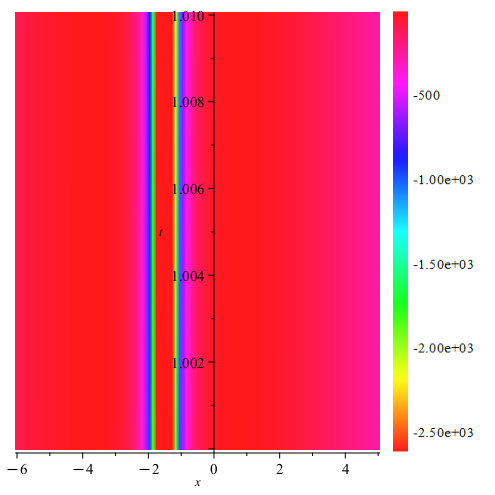
\includegraphics[width=\linewidth, height=35mm]{d9.png}\subcaption{} \end{minipage}
    \end{tabular}%
 \noindent\caption{\ref{U555} yields the 3D and density plot of $U_5(\xi)$ which are displayed here.}\label{F9}
\end{figure}
\FloatBarrier
\section{Results and Discussion}\label{s4}
Analytical soliton  are analyzed utilizing robust integration techniques (unified) which is new and distinct from results obtained by using other approaches. The following observations are provided by using the suitable values for the unknown coefficients and regular measurements to describe the visual result of these  with three dimensional and two dimensional density graphs. The 3D and density plots are used to explore physical phenomena of our observations, the observations are as follows: Fig. (\ref{F1}) and Fig. (\ref{F2}) depict the periodic waves of the Eq. \ref{U1} and Eq. \ref{U2} . Fig. (\ref{F3},\ref{F5},\ref{F8}) and Fig. (\ref{F9}) depict the dark solitons of the Eq. \ref{U4}, \ref{U44}, \ref{U222} and Eq. \ref{U555} . The kink shaped wave profile for the solution of Eq. \ref{U33} is shown in Fig. (\ref{F4}). The anti-Kink shaped soliton of solution of Eq. \ref{U111} is displayed in Fig. (\ref{F7}). A dispersion-less soliton of solution of Eq. \ref{U55} is shown in Fig. (\ref{F6}). As a result, we used Maple software to analyze the answers we found by converting them back to the original Boussinesq equation using mathematical symbols.

\section{Conclusion}\label{s5}
\noindent This paper proposes a Unified approach technique to solve the ill-possed Boussinesq equation and produces different new  and the  we obtained from the unified approach method has not been published yet. Also, these new  may provide us with the current findings and aid in providing much greater clarity for the equations physical characteristics. Using Maple software, the  are obtained. This method is very general as well as simple and easy for finding the exact  of non-linear partial differential equations which shows the efficiency, productivity and suitability of this method for handling many other non-linear partial differential equations (NPDE's)
\begin{thebibliography}{99}

\bibitem{aty1} Abdel-Aty, M., Abdel-Khalek, S., Obada, A.-S.F.
Pancharatnam phase of two-mode optical fields with Kerr nonlinearity, Optical Review, 2000, 7(6), pp. 499--504 DOI: \url{http://dx.doi.org/10.1007/s10043-000-0499-6}

\bibitem{aty2} Rehman, H.U., Said, G.S., Amer, A., Elazab, N.S., Osman, M.S.
Unraveling the (4+1)-dimensional Davey-Stewartson-Kadomtsev-Petviashvili equation: Exploring soliton  via multiple techniques, Alexandria Engineering Journal, 2024, 90, pp. 17--23 DOI: \url{http://dx.doi.org/10.1016/j.aej.2024.01.058}

\bibitem{aty3} Abdel-aty, M.
Quantum field entropy and entanglement of a three-level atom two-mode system with an arbitrary nonlinear medium, Journal of Modern Optics, 2003, 50(2), pp. 161--177 DOI: \url{http://dx.doi.org/10.1080/09500335308235167}

\bibitem{aty4} El-Shahat, T.M., Abdel-Khalek, S., Abdel-Aty, M., Obada, A.-S.F.
Aspects on entropy squeezing of a two-level atom in a squeezed vacuum, Chaos Solitons and Fractals, 2003, 18(2), pp. 289--298 DOI: \url{http://dx.doi.org/10.1016/S0960-0779(02)00652-5}

\bibitem{aty5} Obada, A.-S.F., Abdel-Aty, M.
Influence of the stark shift and kerr-like medium on the evolution of field entropy and entanglement in two-photon processes, Acta Physica Polonica B, 2000, 31(3), pp. 589--599 URL: \url{https://www.actaphys.uj.edu.pl/fulltext?series=Reg&vol=31&page=589}

\bibitem{aty6} Abdel-Aty, M., Abdalla, M.S., Obada, A.-S.F.
Entropy and phase properties of isotropic coupled oscillators interacting with a single atom: one- and two-photon processes, Journal of Optics B Quantum and Semiclassical Optics, 2002, 4(3), pp. S133--S141 DOI: \url{http://dx.doi.org/10.1088/1464-4266/4/3/367}

\bibitem{aty7} Zhang, J.-S., Chen, A.-X., Abdel-Aty, M.
Two atoms in dissipative cavities in dispersive limit: Entanglement sudden death and long-lived entanglement, Journal of Physics B Atomic Molecular and Optical Physics, 2010, 43(2), 025501 DOI: \url{http://dx.doi.org/10.1088/0953-3575/43/2/025501}

\bibitem{aty8} Sebawe Abdalla, M., Hassan, S.S., Abdel-Aty, M.
Entropic uncertainty in the Jaynes-Cummings model in presence of a second harmonic generation, Optics Communications, 2005, 244(1-6), pp. 431--443 DOI: \url{http://dx.doi.org/10.1016/j.optcom.2004.09.051}

\bibitem{aty9} Abdel-Aty, M.
An investigation of entanglement and quasiprobability distribution in a generalized Jaynes-Cummings model, Journal of Mathematical Physics, 2003, 44(4), pp. 1457--1471 DOI: \url{http://dx.doi.org/10.1063/1.1559643}

\bibitem{aty10} Abdel-Aty, M., Sebawe Abdalla, M., Obada, A.-S.F.
Entropy squeezing of a two-mode multiphoton Jaynes-Cummings model in the presence of a nonlinear medium, Journal of Optics B Quantum and Semiclassical Optics, 2002, 4(2), pp. 134--142 DOI: \url{http://dx.doi.org/10.1088/1464-4266/4/2/309}

\bibitem{A1} Anil Sezer, S., Yildirim, A. and Tauseef Mohyud-Din, S. (2011). He's homotopy perturbation method for solving the fractional KdV-Burgers-Kuramoto equation. \emph{International Journal of Numerical Methods for Heat and Fluid Flow, 21}(4), 448-458. DOI: \url{https://doi.org/10.1108/09615531111123119}

\bibitem{A2} Tauseef Mohyud-Din, S., Aslam Noor, M., Noor, K.I. and Hosseini, M.M. (2010). Variational iteration method for re-formulated partial differential equations. \emph{International Journal of Non-linear Sciences and Numerical Simulation, 11}(2), 87-92. DOI: \url{https://doi.org/10.1515/IJNSNS.2010.11.2.87}

\bibitem{A3} Shakeel, M. and Mohyud-Din, S.T. (2015). Improved (G'/G)-expansion and extended tanh methods for (2+ 1)-dimensional Calogero-Bogoyavlenskii-Schiff equation. \emph{Alexandria Engineering Journal, 54}(1), 27-33. DOI: \url{https://doi.org/10.1016/j.aej.2014.11.003}

\bibitem{a4} Guner, O., Atik, H. and Kayyrzhanovich, A.A. (2017). New exact solution for space-time fractional differential equations via (G'/G)-expansion method. \emph{Optik-Internatinal Journal for Light and Electron Optics, 130}, 696-701. DOI: \url{https://doi.org/10.1016/j.ijleo.2016.10.116}

\bibitem{a5} Ekici, M. (2017). Soliton and other  of non-linear time fractional parabolic equations using extended G'/G-expansion method. \emph{Optik, 130}, 1312-1319. DOI: \url{https://doi.org/10.1016/j.ijleo.2016.11.135}

\bibitem{a6} Guner, O., Bekir, A. and Bilgil, H. (2015). A note on exp-function method combined with complex transform method applied to fractional differential equations. \emph{Advances in Nonlinear Analysis, 4}(3), 201-208. DOI: \url{https://doi.org/10.1515/anona-2015-0019}

\bibitem{a7} Navickas, Z., Telksnys, T. and Ragulskis, M. (2015). Comments on -the exp-function method and generalized solitary -. \emph{Computers and Mathematics with Applications, 69}(8), 798-803. DOI: \url{https://doi.org/10.1016/j.camwa.2015.02.017}

\bibitem{a8} Noor, M.A., Mohyud-Din, S.T. and Waheed, A. (2009). Exp-function method for solving Kuramoto-Sivashinsky and Boussinesq equations. \emph{Journal of Applied Mathematics and Computing, 29}, 1-13. DOI: \url{https://doi.org/10.1007/s12190-008-0083-y}

\bibitem{a9} Mohyud-Din, S.T., Noor, M. A. and Waheed, A. (2009). Exp-function method for generalized traveling  of good Boussinesq equations. \emph{Journal of Applied Mathematics and Computing, 30}, 439-445. DOI: \url{https://doi.org/10.1007/s12190-008-0183-8}

\bibitem{a10} Younis, M. and Zafar, A. (2013). The modified simple equation method for solving nonlinear Phi-Four equation. \emph{International Journal of Innovation and Applied Studies, 2}(4), 661-664. URL: \url{https://ijias.issr-journals.org/abstract.php?article=IJIAS-13-046-01}

\bibitem{a11} Zayed, E.M. (2011). A note on the modified simple equation method applied to Sharma-Tasso-Olver equation. \emph{Applied Mathematics and Computation, 218}(7), 3962-3964. DOI: \url{https://doi.org/10.1016/j.amc.2011.09.027}

\bibitem{a12} El-Wakil, S.A. and Abdou, M.A. (2007). New exact travelling wave  using modified extended tanh-function method. \emph{Chaos, Solitons and Fractals, 31}(4), 835-852. DOI: \url{https://doi.org/10.1016/j.chaos.2005.10.032}

\bibitem{a13} Xu, T., Li, J., Zhang, H.Q., Zhang, Y. X., Yao, Z. Z. and Tian, B. (2007). New extension of the tanh-function method and application to the Whitham-Broer-Kaup shallow water model with symbolic computation. \emph{Physics Letters A, 369}(5-6), 458-463. DOI: \url{https://doi.org/10.1016/j.physleta.2007.05.008}

\bibitem{a14} Inc, M. and Fan, E.G. (2005). Extended tanh-function method for finding travelling wave  of some non-linear partial differential equations. \emph{Zeitschrift f-r Naturforschung A, 60}(1-2), 7-16. DOI: \url{https://doi.org/10.1515/zna-2005-1-202}

\bibitem{a15} Hosseini, K., Bekir, A. and Ansari, R. (2017). New exact  of the conformable time-fractional Cahn-Allen and Cahn-Hilliard equations using the modified Kudryashov method. \emph{Optik, 132}, 203-209. DOI: \url{https://doi.org/10.1016/j.ijleo.2016.12.029}

\bibitem{a16} Kaplan, M., Bekir, A. and Akbulut, A. (2016). A generalized Kudryashov method to some non-linear evolution equations in mathematical physics. \emph{Non-linear Dynamics, 85}, 2843-2850. DOI: \url{https://doi.org/10.1007/s11071-016-2867-1}

\bibitem{a17} Gurefe, Y., Misirli, E., Sonmezoglu, A. and Ekici, M. (2013). Extended trial equation method to generalized non-linear partial differential equations. \emph{Applied Mathematics and Computation, 219}(10), 5253-5260. DOI: \url{https://doi.org/10.1016/j.amc.2012.11.046}

\bibitem{a18} Ghosh, S. and Nandy, S. (1999). Inverse scattering method and vector higher order non-linear Schr-dinger equation. \emph{Nuclear Physics B, 561}(3), 451-466. DOI: \url{https://doi.org/10.1016/S0550-3213(99)00484-8}

\bibitem{a19} Ma, W.X. and Abdeljabbar, A. (2012). A bilinear B-cklund transformation of a (3+ 1)-dimensional generalized KP equation. \emph{Applied Mathematics Letters, 25}(10), 1500-1504. DOI: \url{https://doi.org/10.1016/j.aml.2012.01.003}

\bibitem{a20} Wazwaz, A.M. (2008). The Hirota-s bilinear method and the tanh-coth method for multiple-soliton  of the Sawada-Kotera-Kadomtsev-Petviashvili equation. \emph{Applied Mathematics and Computation, 200}(1), 160-166. DOI: \url{https://doi.org/10.1016/j.amc.2007.11.001}

\bibitem{a21} Wang, M., Zhou, Y. and Li, Z. (1996). Application of a homogeneous balance method to exact  of non-linear equations in mathematical physics. \emph{Physics Letters A, 216}(1-5), 67-75. DOI: \url{https://doi.org/10.1016/0375-9601(96)00283-6}

\bibitem{a22} Liu, S., Fu, Z., Liu, S. and Zhao, Q. (2001). Jacobi elliptic function expansion method and periodic wave  of nonlinear wave equations. \emph{Physics Letters A, 289}(1-2), 69-74. DOI: \url{https://doi.org/10.1016/S0375-9601(01)00580-1}

\end{thebibliography}
\end{document}
